% !TEX TS-program = pdflatex
% !TEX encoding = UTF-8 Unicode

% This is a simple template for a LaTeX document using the "article" class.
% See "book", "report", "letter" for other types of document.

\documentclass[12pt]{article} % use larger type; default would be 10pt






%%% PAGE DIMENSIONS
\usepackage{makeidx}
\usepackage{hyperref}
\usepackage[margin=0.75in]{geometry} % to change the page dimensions
\geometry{a4paper} % or letterpaper (US) or a5paper or....

\usepackage[pdftex]{graphicx} % support the \includegraphics command and options

\usepackage{array} % for better arrays (eg matrices) in maths
\usepackage{verbatim} % adds environment for commenting out blocks of text & for better verbatim
%\usepackage{subfig} % make it possible to include more than one captioned figure/table in a single float
% These packages are all incorporated in the memoir class to one degree or another...

%%% HEADERS & FOOTERS
\usepackage{fancyhdr} % This should be set AFTER setting up the page geometry


\newcommand{\HRule}{\rule{\linewidth}{0.5mm}}


\begin{document}
\maketitle

\begin{titlepage}

\begin{center}


% Upper part of the page

\includegraphics[scale=0.75]{RVCE.png}\\[1cm]    

\textsc{\LARGE  RV College of Engineering}\\[0.5cm]
\large{Department of Computer Science}\\[1cm]
\textsc{\Large }\\[0.5cm]

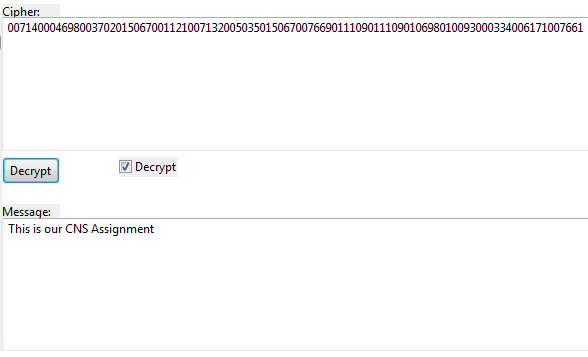
\includegraphics[scale=0.75]{proj.png}\\[1cm]    

% Title
\HRule \\[0.4cm]
{  \huge\bfseries Schmidt-Samoa Cryptosystem }\\[0.4cm]

\HRule \\[1cm]

% Author and supervisor
\begin{minipage}{0.8\textwidth}
\begin{flushleft} \large
\emph{By:}\\
Satvik \textsc{N} [1RV09CS095]\\
Vaishakh \textsc{BN} [1RV09CS114]\\

\end{flushleft}
\end{minipage}
\vfill

% Bottom of the page
{\large}

\end{center}

\end{titlepage}



\maketitle
\setcounter{secnumdepth}{1}

\section{Introduction}
Public-key cryptography refers to a cryptographic system requiring two separate keys, one of which is secret and one of which is public. Although different, the two parts of the key pair are mathematically linked. One key locks or encrypts the plaintext, and the other unlocks or decrypts the ciphertext. Neither key can perform both functions. One of these keys is published or public, while the other is kept private.
\subsection{How Pubic-key Cryptosystems Work}
The distinguishing technique used in public-key cryptography is the use of asymmetric key algorithms, where the key used to encrypt a message is not the same as the key used to decrypt it. Each user has a pair of cryptographic keys - a public encryption key and a private decryption key. The publicly available encrypting-key is distributed, while the private decrypting-key is kept secret. Messages are encrypted with the recipient's public key, and can be decrypted only with the corresponding private key. The keys are related mathematically, but the parameters are chosen so that determining the private key from the public key is either impossible or prohibitively expensive. 


\subsection{Schmidt-Samoa Public-key Cryptosystem}
The Schmidt-Samoa cryptosystem is an asymmetric cryptographic technique, whose security, like Rabin and RSA depends on the difficulty of integer factorization.
\begin{itemize}
\item{Key generation}
\begin{itemize}
\item{}Choose two large distinct primes p and q and compute $N = p^2 \times q$
\item{}Compute $d = N-1$ mod $lcm(p - 1, q - 1)$
\item{}Now N is the public key and d is the private key.
 \end{itemize}


\item{\textbf{Encryption}} - 
To encrypt a message m we compute the cipher text as $c = m^N mod N$
 
\item{\textbf{Decryption}}
To decrypt a cipher text c we compute the plaintext as $m = c^d mod (p\times q)$ which like for Rabin and RSA can be computed with the Chinese remainder theorem.



\item{\textbf{Security}} - 
The algorithm, like Rabin, is based on the difficulty of factoring the modulus N, which is a distinct advantage over RSA. That is, it can be shown that if there exists an algorithm that can decrypt arbitrary messages, then this algorithm can be used to factor N.
\end{itemize}

\section{Previous Cryptosystems}
\subsection{RSA Cryptosystem}
RSA stands for Ron Rivest, Adi Shamir and Leonard Adleman, who first publicly described it in 1977.

\begin{itemize}
\item{\textbf{Key Generation}}
\begin{itemize}
\item{}Let N = pq be a product of two prime numbers
\item{}Compute $φ(n) = (p – 1)(q – 1)$, where φ is Euler's totient function.
\item{}Choose an integer e such that 1 < e < φ(n) and greatest common divisor of (e, φ(n)) = 1; i.e., e and φ(n) are coprime.
\item{}Determine d as: d º e-1 (mod φ(n)) i.e., d is the multiplicative inverse of e mod φ(n).
 \end{itemize}

\item{\textbf{Encryption}}:    Let M be a message, and c the ciphertext. Then,
        	$c = m^e (mod n)$
\item{\textbf{Decryption}}:  $m = c^d (mod n)$
By construction, d*e= 1 mod φ(n). The public key consists of the modulus n and the public (or encryption) exponent e. The private key consists of the modulus n and the private (or decryption) exponent d which must be kept secret.
\end{itemize}
\subsection{Rabin’s Cryptosystem}
In 1979, Michael Rabin suggested a variant of RSA with public-key exponent 2, which he showed to be as secure as factoring.
Let N = pq be a product of two prime numbers.
Encryption. Let m∈   ZNx, M be a message, the encryption is
C = m2 mod N
Decryption. To decrypt we solve the equation
x2 = C mod N
which has four roots in ZNx



\section{Implementation}
It's all yours!





%\begin{figure}[h!]
%  \centering
%   \includegraphics[scale=0.50]{watlas.png}
%  \caption{A small portion of the Watershed Atlas for British Columbia that was
%developed using an IBM Informix ORDBMS.}
%\end{figure}


\newpage

\begin{thebibliography}{9}
\bibitem{pap}
Katja Schmidt-Samoa, 
\emph{A New Rabin-type Trapdoor Permutation Equivalent to Factoring and Its Applications}. TechnischeUniversit. samoa@informatik.tu-darmstadt.de

\bibitem{wiki}
  Schmidt-Samoa Cryptosystem - 
 \url{http://en.wikipedia.org/wiki/Schmidt-Samoa_cryptosystem}
\bibitem{textbook}
 Rivest, R.; A. Shamir; L. Adleman (1978). \emph{"A Method for Obtaining Digital Signatures and Public-Key Cryptosystems"}. Communications of the ACM 21 (2): 120–126. doi:10.1145/359340.359342

\bibitem{pdp} Joe Hurd, Blum Integers (1997) -  \url{http://www.gilith.com/research/talks/cambridge1997.pdf}
\bibitem{pap}Rabin, Michael. \emph{Digitalized Signatures and Public-Key Functions as Intractable as Factorization}. MIT Laboratory for Computer Science, January 1979.

\bibitem{link}Katja Schmidt-Samoa - \emph{Contributions to Provable Security and Efficient Cryptography}.\\\url{http://tuprints.ulb.tu-darmstadt.de/708/1/Diss.Schmidt-Samoa.pdf}
\end{thebibliography}
\section{Screenshots}
\begin{figure}[h!]
  \centering
   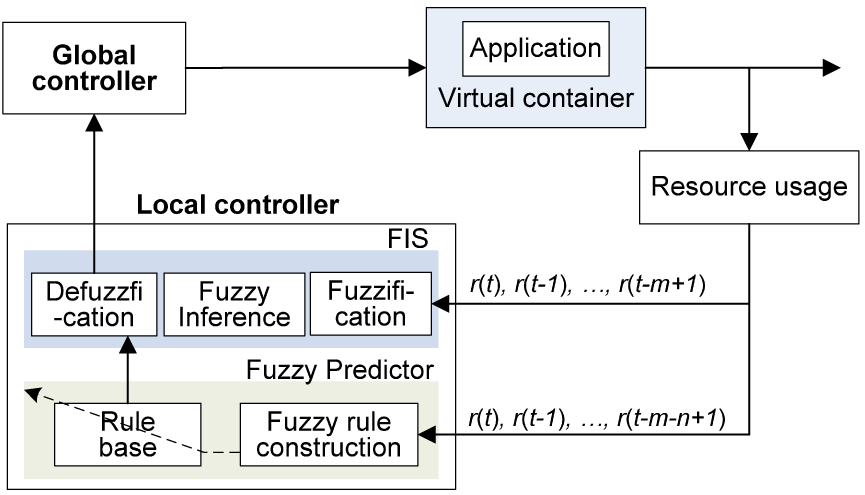
\includegraphics[scale=0.50]{fuzzy_block_dia.png}
  \caption{Resource management based on fuzzy logic systems.}
\end{figure}

\begin{figure}[h!]
  \centering
   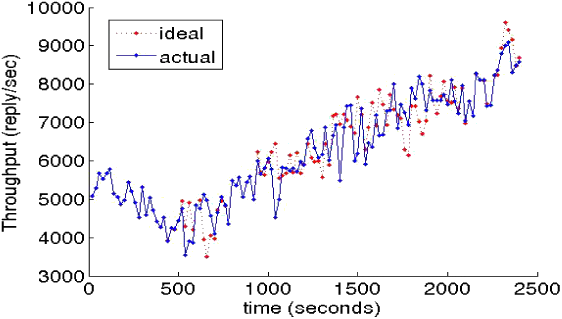
\includegraphics[scale=0.50]{fuzzy_experiment.png}
  \caption{Experimental Results}
\end{figure}
\begin{figure}[h!]
  \centering
   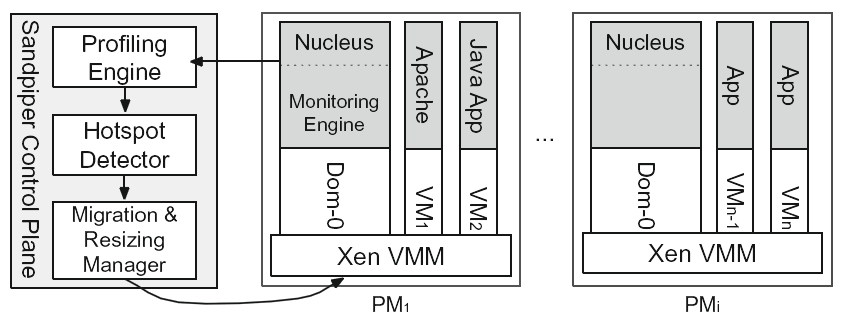
\includegraphics[scale=0.60]{sandpiper_arch.png}
  \caption{The Sandpiper architecture.}
\end{figure}

\end{document}
